\chapter{Implementation}
	
	Due to MediaWiki being written in PHP and requiring its extensions to be in the same language to use its functionality, the core part of the ArticlePlaceholder extension is written in PHP, too. The programming language PHP is ``a popular general-purpose scripting language that is especially suited to web development.'' \footnote{http://php.net/} \\
	Therefore all parts, that need some services or work with the functionality of MediaWiki must be written in PHP- such as the special page for users to create an ArticlePlaceholder as well as the integration in the search page. \\
	The ordering of statement groups is written mainly in PHP to be reusable. It could have been implemented in Lua, too, but then would have been almost exclusively useful for this extension. \\
	The layout and display of the item on the Wikipedia, the core part from a users perspective, is realized with a Lua module. This module takes the function of a library by being able to be overwritten by users with setter functions and having getter functions. It is called from the special page with a Template -- \texttt{Template:AboutTopic} -- which itself contains only the call to the \texttt{Module:AboutTopic} Lua module's function \texttt{showData}. The named template and module are on the respective Wikipedia. \\

	\section{Setting up the extension}
	To enable and setup an extension in MediaWiki, the extension has to have a file called \texttt{\justify ExtensionName.php}, which in this case would be \texttt{\justify ArticlePlaceholder.php}. \texttt{\justify ArticlePlaceholder.php} stores the setup instructions and contains declarations and definitions important to this extension. \\
	To register the extension in MediaWiki, in the file \texttt{\justify LocalSettings.php} the ArticlePlaceholder is set with \texttt{\justify require\_once( ``\$IP/extensions/ArticlePlaceholder/ArticlePlaceholder.php'' );}. \\
	Additionally the extension registration has the global variable \texttt{\justify \$wgArticlePlaceholderImageProperty}. This is needed for the user installing the extension to set the image property of their repository. In the case of Wikidata this would be \textit{``image'' (P18)}. \citep{wiki:23}
	\section{SpecialPage}

The SpecialPage \texttt{\justify Special:AboutTopic} uses multiple services provided either by Wikibase or MediaWiki. It also extends the class \texttt{\justify SpecialPage} provided by MediaWiki. The class is called \texttt{\justify SpecialAboutTopic} and can be found in the namespace \texttt{\justify ArticlePlaceholder\textbackslash{}Specials}. \\
The SpecialPage serves two purposes: It creates the form for the SpecialPage itself, and is used to display the ArticlePlaceholder. \\
From a user's perspective there are two ways of passing an entity ID to the extension. 
The first option is to enter the ID on the SpecialPage. The SpecialPage is created by an HTML form in the function \texttt{\justify createForm()}, which adds HTML to the \texttt{\justify OutputPage} object provided by MediaWiki. \\
When the entity ID is passed, there is a check with the \texttt{\justify EntityLookup} provided by Wikibase whether this entity actually exists. \\ 
If the entity ID does not exist, the user will get the form again with an additional error message. \\
\\
The second option to get to an ArticlePlaceholder is to pass the ID directly via the URL, for example in the following way.
\begin{center}
\colorbox{Gray}{\lstinline[basicstyle=\ttfamily\color{white}]|Special:AboutTopic/Q5279|}
\end{center}

If the entity ID exists, the SpecialPage needs to check with the \texttt{\justify SiteLinkLookup} service by Wikibase whether there is already an article on this wiki for the item. The function \texttt{\justify getArticleOnWiki( \$entityId)} is called. When an article exists, it returns the title of that article. The user is then forwarded to that article with the \texttt{\justify redirect( \$url )} function of the \texttt{\justify OutputPage} class.
The flowchart for the described code can be seen in Figure~\ref{fig:createpl}. 
\begin{figure}[H]
	\centering
	\tikzstyle{block} = [rectangle, draw, 
    text width=5em, text centered, rounded corners, minimum height=4em]
\tikzstyle{error} = [draw, ellipse, node distance=3cm,
    minimum height=2em]
\tikzstyle{line} = [draw, -latex']
\tikzstyle{cloud} = [draw, ellipse, node distance=3cm,
    minimum height=2em]
\tikzstyle{final} = [diamond, draw, 
    text width=4.5em, text badly centered, node distance=3cm, inner sep=0pt]

\sffamily

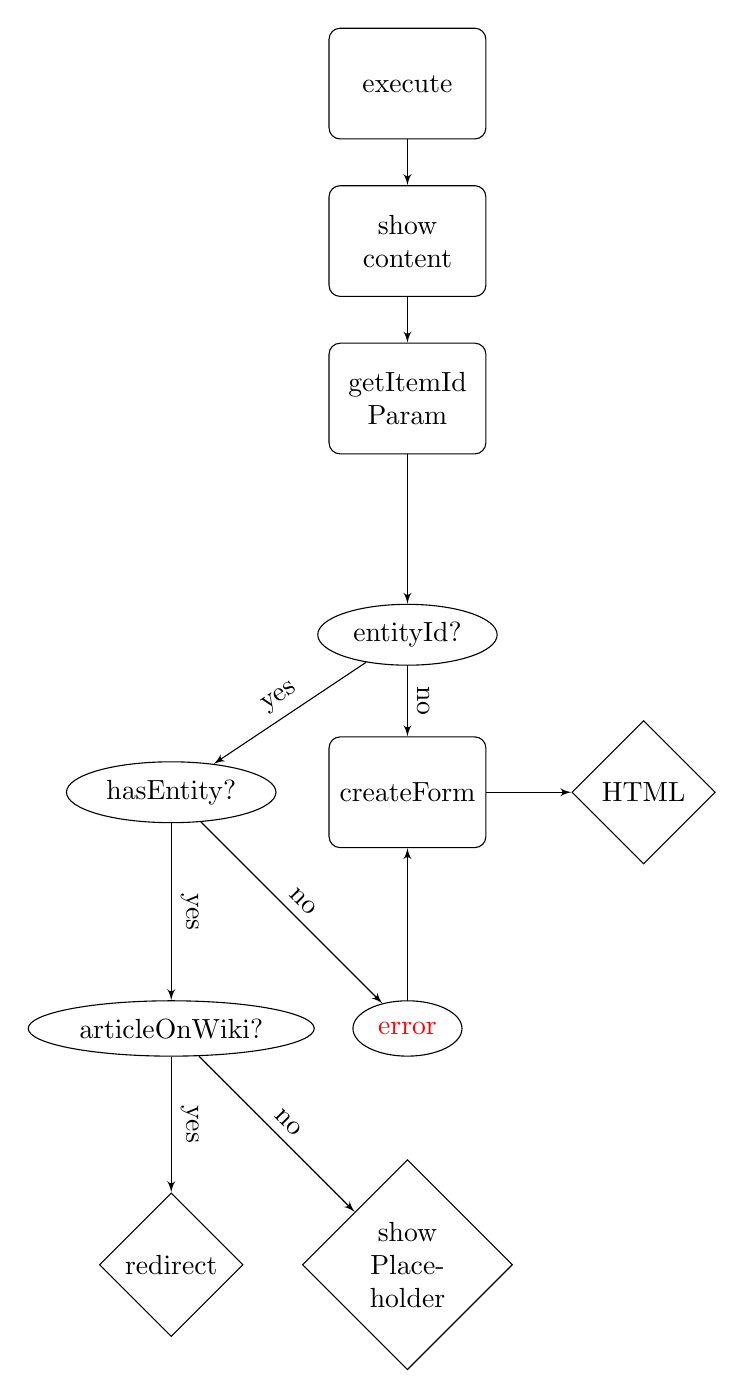
\begin{tikzpicture}[node distance = 2cm, auto]
    % Place nodes
    \node [block] (execute) {execute};
    \node [block, below of=execute] (showContent){show content};
    \node [block, below of=showContent] (itemIdParam) {getItemId Param};
    \node [cloud, below of=itemIdParam] (entityId) {entityId?};  
    \node [block, below of=entityId] (createForm) {createForm};
    \node [final, right of=createForm] (Html) {HTML};
    \node [cloud, left of=createForm] (hasEntity) {hasEntity?};
    \node [cloud, below of=hasEntity] (onWiki) {articleOnWiki?};
    \node [error, right of=onWiki] (error) {\textcolor{red}{error}};
    \node [final, below of=onWiki] (redirect) {redirect};
    \node [final, right of=redirect] (placeholder) {show Placeholder};
    % \node [final, right of=placeholder] (JS) {JavaScript};
    % Draw edges
    \path [line] (execute) -- (showContent);
    \path [line] (showContent) -- (itemIdParam);
    \path [line] (itemIdParam) -- (entityId);
    % \path [line] (entityId) -- (createForm);
    \path [line] (entityId) -- (createForm) node [midway, above, sloped, -latex'] (textnode) {no};
    \path [line] (createForm) -- (Html);
    \path [line] (entityId) -- (hasEntity) node [midway, above, sloped, -latex'] (textnode) {yes};
    % \path [line] (entityId) -- (hasEntity);
    \path [line] (hasEntity) -- (onWiki) node [midway, above, sloped, -latex'] (textnode) {yes};
    %\path [line] (hasEntity) -- (onWiki);
    \path [line] (hasEntity) -- (error) node [midway, above, sloped, -latex'] (textnode) {no};
    % \path [line] (hasEntity) -- (error);
    \path [line] (error) -- (createForm);
    \path [line] (onWiki) -- (redirect) node [midway, above, sloped, -latex'] (textnode) {yes};
    % \path [line] (onWiki) -- (redirect);
    \path [line] (onWiki) -- (placeholder) node [midway, above, sloped, -latex'] (textnode) {no};
    % \path [line] (onWiki) -- (placeholder);
    % \path [line] (placeholder) -- (JS);
\end{tikzpicture}

\rmfamily
	\caption{Flowchart: ArticlePlaceholder creation}
	\label{fig:createpl}
\end{figure}

If there is no article for the passed item, then an ArticlePlaceholder is created. In order to do this, a template on the wiki is invoked, which calls the Lua module. Additionally \texttt{\justify OOUI} is enabled, which is needed for the button creation in PHP. The label of the item is passed to the JavaScript module \texttt{\justify ext.articleplaceholder.createArticle}. The label is used in PHP also to set the title of the page. Links to other Wikipedia language versions (language links) are set in PHP. The sitelinks are read from the \texttt{\justify SiteStore} service provided by Wikibase. They are constructed by combining the language code and the page name, with a colon in between. For example, the page linking to English Wikipedia article on ``Ada Lovelace'' would be \texttt{\justify en:Ada Lovelace}.\\
Showing a placeholder can be described as in Figure~\ref{fig:showpl}. 
\begin{figure}[H]
	\centering
	\tikzstyle{block} = [rectangle, draw, 
    text width=5em, text centered, rounded corners, minimum height=4em]
\tikzstyle{line} = [draw, -latex']

\sffamily

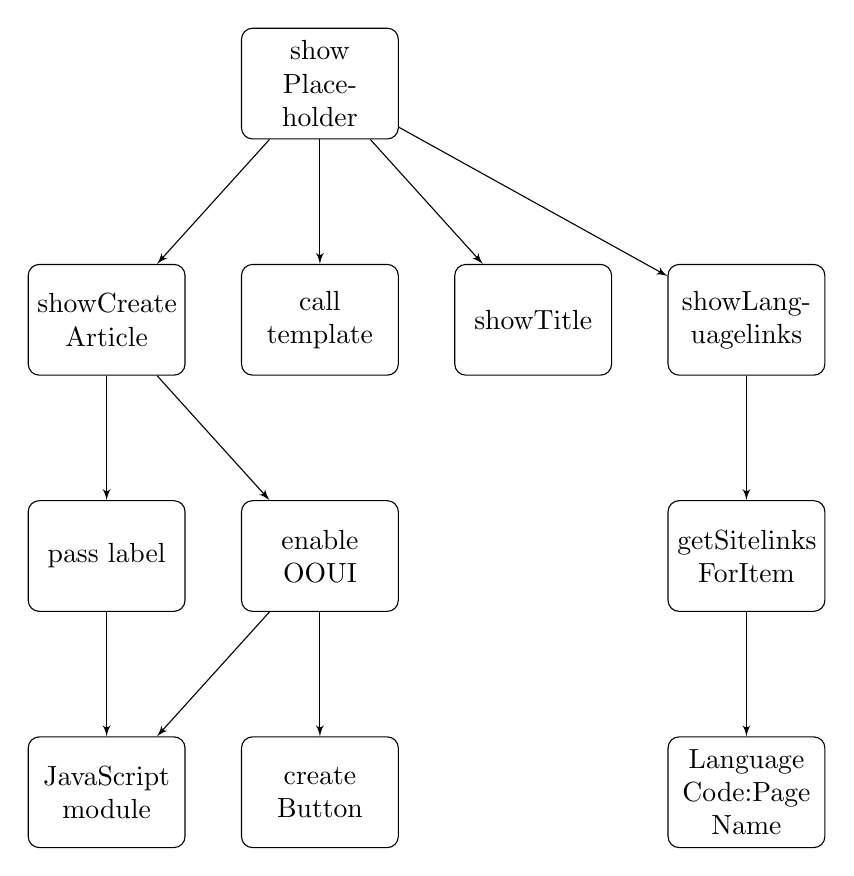
\begin{tikzpicture}[node distance = 3cm, auto]
    % Place nodes
    \node [block, align=center] (showPl) {show Placeholder};
    \node [block, below of=showPl] (callTemp) {call template};
    \node [block, left=2em of callTemp] (showCA){showCreate Article};
	\node [block, right=2em of callTemp] (showTitle) {showTitle};
	\node [block, right=2em of showTitle] (showLl) {showLang-uagelinks};
	\node[block, below of=showCA] (passL) {pass label};
	\node [block, right=2em of passL] (enableOOUI) {enable OOUI};
	\node [block, below of=passL] (JS) {JavaScript module};
	\node [block, right=2em of JS] (createB) {create Button};
	\node [block, below of=showLl] (sl) {getSitelinks ForItem};
	\node [block, below of=sl] (lcpn) {Language Code:Page Name};
	
    % Draw edges
    \path [line] (showPl) -- (showCA);
	\path [line] (showPl) -- (callTemp);
	\path [line] (showPl) -- (showTitle);
	\path [line] (showPl) -- (showLl);
	\path [line] (showCA) -- (enableOOUI);
	\path [line] (showCA) -- (passL);
	\path [line] (enableOOUI) -- (createB);
	\path [line] (enableOOUI) -- (JS);
	\path [line] (passL) -- (JS);
	\path [line] (showLl) -- (sl);
	\path [line] (sl) -- (lcpn);
\end{tikzpicture}

\rmfamily
	\caption{Flowchart: Showing an ArticlePlaceholder}
	\label{fig:showpl}
\end{figure}

	\newpage
\section{Display}
	The display is one of the main parts of the ArticlePlaceholder, as it is user-facing and therefore needs an initial default design. \\
	\begin{figure}[H]
		\centering
		\includegraphics[width=\textwidth]{diagrams/Screenshot-ArticlePlaceholder.png}
		\caption{Screenshot of the ArticlePlaceholder layout as of January 2016}
		\label{screenshot}
	\end{figure}
	The core part of the page is formed by the statement groups. These consist of a property, one or multiple values, and their qualifiers. \\
	Each statement group is in a box with a black border and arranged in a tile layout. The number of statement boxes per row differs depending on the width of the screen. \\
	\begin{figure}[H]
		\centering
		\includegraphics[width=\textwidth]{diagrams/references.png}
		\caption{Screenshot of the ArticlePlaceholder layout, Reference section as of January 2016}
		\label{fig:references}
	\end{figure}
	The main image of the item is on the right side (for left to right languages) of the page, where it would also be in articles.\\
	The label of the property is the header for each group, which is separated from the body by a horizontal line. Multiple values for the same statement are listed. Their qualifiers are directly under the corresponding value in a smaller font size. \\
	References can be found in their own section at the bottom of the page, conforming to the existing layout of Wikipedia, see Figure~\ref{fig:references}. \\
	The identifiers of an item should be in a distinct position so as to be both emphasized and distinguishable from the other statements. They are listed below the main image of the article to the right of the statement groups.
	
	\subsection{Renderer}

Every part of an entity, or item in the case of the ArticlePlaceholder, needs a \textit{renderer} to be displayed. The renderer pulls data from Wikidata and renders it to HTML. It sets CSS classes for the HTML elements in order to style them with the CSS module \texttt{\justify ext.articleplaceholder.defaultDisplay.css}. The HTML output of the module is displayed on the \texttt{\justify Special:AboutTopic} ArticlePlaceholder. \\
The MediaWiki conventions for naming Lua modules is 
\begin{center}
\texttt{\justify mw.ext.extensionName.moduleName} 
\end{center}
In order to match them, the renderer for the ArticlePlaceholder is called 
\begin{center}
\texttt{\justify mw.ext.articlePlacholder.entityRenderer}
\end{center}
Every renderer has getter and setter functions. Therefore every part of the display can be overwritten locally on Wikipedia. \\
The Lua module on the Wikipedia is on the page \texttt{\justify Module:AboutTopic}, which is called by the template \texttt{\justify Template:AboutTopic}. In the module AboutTopic a user with the appropriate rights can call the get and set functions. \\
The renderer are as decoupled as possible so that for example the \texttt{\justify snaksRenderer} can be used by the \texttt{\justify refererenceRenderer} as well as the \texttt{\justify qualifierRenderer}. \\
The Wikibase client provides a Scribunto interface with modules to access the repository. Wherever possible, the functions provided by this interface were used. This way, the description renderer for example simply calls \texttt{\justify mw.wikibase.description} and passes the entity Id as a parameter. The \texttt{\justify descriptionRenderer} of the ArticlePlacheolder's EntityRenderer is still needed since there must be a possibility for the user to overwrite the renderer. Additionally a CSS class needs to be assigned to the result of Wikibase's description renderer in order to style it properly. \\
The EntityRenderer module itself takes just the entity Id of an item an ArticlePlaceholder is created for. The Lua table for an entity is loaded in the renderEntity function. This table represents a whole entity with all its respective data. Therefore it is performance-wise the most expensive operation in the module. \\

\begin{figure}[H]
	\centering
	\includegraphics[width=\textwidth]{diagrams/EntityRendererMethods.png}
	\caption{Diagram of all renderer functions}
	\label{fig:renderer}
\end{figure}

\todo[inline]{3 examples, one easy, two tricky, ``additionally there are renderer for ...'' and digram}
	\subsubsection{Identifier}

To get a list of all external identifier in Wikidata, the item Q19847637, "Wikidata property representing a unique identifier", is used. To get all the Items, that are an instance of (property P31) this item \href{https://query.wikidata.org}{Wikidata's SPARQL endpoint} is used. With the following query it is possible to download a file with the query result in JSON. \\

\begin{lstlisting}[frame=single] 
PREFIX wd: <http://www.wikidata.org/entity/>
PREFIX wdt: <http://www.wikidata.org/prop/direct/>

SELECT ?identifier WHERE {
   ?identifier  wdt:P31 wd:Q19847637 . 
}
\end{lstlisting}

In a Lua script (Main.lua), the JSON output is converted to another Lua Script. Identifier.lua is generated and returns a Lua table, which contains tables with the Identifier mapped to "true" to be able to check whether a property is an identifier or not. This new script is just included in the Lua module and is called to get access to the table with the identifier. It is static since it would be too many requests to the SPARQL endpoint to check for every call to the special page again if the data on identifier changed. That implies if something changes with the identifiers on Wikidata or a new one is added the article placeholder doesn't reflect that. \\
This implementation is chosen due to the fact that the Wikidata team is working on a identifier data type, which would make the need for a Lua table with all identifier dispense. As soon as there is a identifier data type, the way of checking a property id could be adjusted to just checking for the data type of the respective property. 

	\documentclass[11pt]{article}

\usepackage[dvipsnames]{xcolor}
\usepackage{hyperref}
\usepackage{todonotes}
\usepackage{listings}
\usepackage{soul}
\usepackage[latin1]{inputenc}
\usepackage{tikz}
\usetikzlibrary{shapes,arrows}

\title {{Implementation}}
\author {Lucie-Aim\'{e}e Kaffee}
\date{}

\begin{document}
Test
\end{document}
	\subsection{Style elements (CSS)}

In order to style the layout elements, CSS classes are assigned in the Lua module. Their looks as well as the create article button's look are adjusted in \texttt{ext.articleplaceholder.defaultDisplay.css}. \\
So as not to conflict with other MediaWiki style elements, the CSS classes are prefixed with \texttt{\justify articleplaceholder-}. \\
The \texttt{\justify divs} are nested so that, for example, the main image and the identifier (which both have their own \texttt{div}) are in one \texttt{div} named after its place in the layout \texttt{\justify articleplaceholder-sidebar}. Additionally the identifiers are all in one \texttt{div}, the \texttt{\justify articleplaceholder-identifierlist}. \\
The \texttt{divs} containing the statement groups have a maximum width, so that a maximum of three boxes are in one row. The number of columns differs depending on the number of statements. When the browser window is smaller, the number of boxes per row adjusts accordingly. Initially it was planned to adjust them to a tiling layout, but since tiling layout in pure CSS would expect the boxes to be ordered vertically in columns this was not possible. \todo{[citation needed]} It is important to show the most important information first, otherwise the ordering of statement groups would be pointless. \\
In order to be responsive, the extension makes use of \textit{media queries}. Media queries are a convenient way to add CSS styles for elements that need to be adjusted for different devices. \citep[43]{mediaquery}\\
In MediaWiki with the \textit{resource loader} \texttt{\justify \$wgResourceModules} media queries can be assigned to CSS modules. This way it is possible to load another CSS module (\texttt{\justify ext.articleplaceholder.defaultDisplaySmall.css}), when the screen size is smaller then 930 pixels. This was added in order to avoid the overlapping of the sidebar with the image and identifiers, and the statement groups.
	\subsection{Search}
In order to be able to find results from the placeholder in the MediaWiki search it was necessary to use the SearchHook provided by MediaWiki.
With the help of the TermSearchInteractor provided by Wikibase, which needed to be moved to Wikibase library in order to be able to use the service in Wikibase client and not only in Wikibase repository as before, all items with labels or aliases matching the given search term are returned. From those a string containing the label of the item, displayed as a link to the special page with the corresponding entity ID, and the description of the item in case there are multiple results.  \\
If the result is not empty, the results are added to the search page as Wikitext. \\
\todo{filtern der Resultate}
\href{https://www.mediawiki.org/wiki/Manual:Hooks/SpecialSearchResultsAppend}{Manual:SpecialSearchResultsAppend}
	\section{Ordering of statement groups}\label{ordering-stat}

To find a technical solution to this problem, there was a "Request for comment" page set up \citep{wiki:24}. \\
\\
The collection of ordered property IDs is stored on one page in the \textit{MediaWiki namespace}. This namespace ``is used to hold system messages and other important content'' \citep{wiki:17}. It can be edited only by administrators. This page is called \texttt{\justify MediaWiki:Wikibase-SortedProperties}. Since the page name is set in the code, it is a constant variable. \\
The code for the ordering is not merged yet, since it's supposed to become part of Wikibase instead of being accessible only in the ArticlePlaceholder extension. That allows the possibility of reusing the code without having to build up a dependency from Wikibase to the  extension. \\
\\
For now, the page has to be on the local Wikipedia. If that's not the case, or if the page is empty or filled with non-text content, the corresponding exception is thrown. For that purpose the \texttt{\justify ArticlePlaceholderException} was created, which extends PHP's \texttt{\justify RuntimeException} to catch more specific exceptions and allow for more specific error handling. \\
In the class \texttt{\justify PropertyOrderProvider} the page is parsed into a PHP array. In this array, the property IDs are the keys and the ordinal numbers the values. \\
\\
To get the content of the page, the MediaWiki function \texttt{\justify getNativeData()} is used. This page content is parsed in the function \texttt{\justify parseList( \$pageContent )}. To remove all comments in the HTML multiple line comment style, the following regular expression is used.
\begin{lstlisting}[frame=single]
@<!--.*?-->@s
\end{lstlisting}
The \texttt{\justify @} is the delimiter. All comments matching this pattern are replaced with empty strings. \\
After removing all comments, all Strings matching the following regular expression are written into an array.
\begin{lstlisting}[frame=single] 
@^\*\s*([Pp]\d+)@m
\end{lstlisting}
This regular expression matches all strings containing an asterisk, optional whitespace, and a upper or lower case \textit{P} followed by a number.
The array is flipped, to have the properties as keys. This is important when it comes to using the array in Lua. It is not used in the \texttt{\justify mw.ext.articlePlaceholder.entityRenderer.lua} module yet, but will be in the future. \\
An instance of the class is created in the \texttt{\justify ArticlePlaceholderServices}. \\
In the class \texttt{\justify Scribunto\_LuaArticlePlaceholderLibrary} in the \texttt{\justify ArticlePlaceholder\textbackslash{}Lua} namespace with the help of \texttt{\justify ArticlePlaceholderServices} the array with the property order is returned in the function \texttt{\justify getPropertyOrder()}, which then can be called in the Lua module. This is explained in further detail in the following Chapter \ref{including-lua}: \nameref{including-lua}. \\
In \texttt{\justify mw.ext.articlePlaceholder.entityRenderer.lua} the property IDs of the item will be ordered according to the ordinal numbers of the sorted array. \\ 
After the sorting is executed, it is quite easy to limit the number of statements, since less important statements can be identified by their ordinal number.
	\subsection{Including Lua}\label{including-lua}
	\section{Internationalization}

The extension includes an \texttt{\justify i18n} folder to be able to localize all strings needed by the extension. This is the way predefined by MediaWiki \citep{wiki:34}.  Every message needed by the extension has a unique message key. These keys are mapped to the text in the different languages. The key-value pairs are stored as JSON. \\
The keys need to be unique not only in the ArticlePlaceholder extension but also must not conflict with MediaWiki's and its other extensions' keys. Therefore they start with \texttt{\justify articleplaceholder-}. Due to MediaWiki conventions, they are all lower case and may not contain spaces. \\
The documentation for every message is stored in the \texttt{\justify qqq.json} file. The other messages are in the JSON files with the appropriate language key. While developing, it is only necessary to define the English and documentation messages, since the other messages are translated by the community on \url{translatewiki.net}.
\begin{quote}
 \citet{wiki:26} states ``\url{translatewiki.net} is a web-based translation platform, powered by the Translate extension for MediaWiki [...] [It has] 6000 translators for over 50[,000] pages from over [twenty] projects including MediaWiki, OpenStreetMap, Mifos, Encyclopedia of Life and MantisBT.''
\end{quote}

To load the messages, their directory is added to \texttt{\justify \$wgMessagesDirs}. \texttt{\justify \$wgMessagesDirs} is an associative array that maps the extension name to the appropriate message directory for the MediaWiki software to extract the messages and their keys. \\
The messages can now be used in PHP, JavaScript and Lua with their respective methods provided by MediaWiki. In PHP the message can be loaded using the function \texttt{\justify wfMessage} with the message key as a parameter. The syntax for Lua is \texttt{\justify mw.message.new( message-key ):plain()} and for JavaScript \texttt{\justify mw.message( message-key ).escaped()}. Due to the similar syntax of Lua and JavaScript, the function call is similar, too. \\ 
In the last two examples, the messages are additionally escaped.
	\section{Unit tests}
	\section{Deployment}
	  \subsubsection{Deployment cycles}
  Since there were different steps of deployments, it was necessary to split up the functional requirements and built up the requirements in every step on the ones before. \\
  The deployment timeline would look like this
  \\ 
  \\
    \begin{tikzpicture}[snake=zigzag, line before snake = 5mm, line after snake = 5mm]
      % draw horizontal line   
      \draw (0,0) -- (2,0);
      \draw[snake] (2,0) -- (4,0);
      \draw (4,0) -- (5,0);
      \draw[snake] (5,0) -- (7,0);
      \draw (7,0) -- (8,0);
	  \draw[snake] (8,0) -- (10,0);
	  \draw (10,0) -- (13.5,0);
      

      % draw vertical lines
      \foreach \x in {0,1.5,4.5,7.5,10.5,12,13.5}
	\draw (\x cm,3pt) -- (\x cm,-3pt);

      % draw nodes
      \draw (0,0) node[below=3pt] {} node[above=3pt] {$   $};
      \draw (1.5,0) node[below=3pt] {\small test system} node[above=3pt] {};
      \draw (3,0) node[below=3pt] {} node[above=3pt] {\small security review};
      \draw (4.5,0) node[below=3pt] {\small beta feature 1} node[above=3pt] {};
      \draw (6,0) node[below=3pt] {} node[above=3pt] {\small feedback};
      \draw (7.5,0) node[below=3pt] {\small beta feature 2} node[above=3pt] {};
      \draw (9,0) node[below=3pt] {} node[above=3pt] {\small feedback};
      \draw (10.5,0) node[below=3pt] {\small deploy WP} node[above=3pt] {};
      \draw (12,0) node[below=3pt] {} node[above=3pt] {\scriptsize more WP deploys};
      \draw (13.5,0) node[below=3pt] {\small sister projects} node[above=3pt] {};
    \end{tikzpicture}

\todo{on own page!}

  \paragraph{Test system}
  To have a possibility to present the extension from the beginning, there was a test setup, available on Wikimedia Labs \footnote{\href{articleplaceholder.wmflabs.org/mediawiki}{articleplaceholder.wmflabs.org/mediawiki}}. Wikimedia Labs is 
	\begin{quotation}
		the Wikimedia Foundation (WMF)'s cloud computing environment for developing software for the Foundation's operations. It also hosts bots and tools maintained and used by the community to maintain the foundation's projects. 
	\end{quotation} \todo{connect to wiki:03}
Besides the bots running on Wikimedia Labs it is used for various tools and to test software by volunteers as well as WMF's staff. \\
The test setup was set up to give editors as well as the public a first insight into what the extension looks like and what it is capable of. It is also aimed at starting a discussion on what can be improved in order to be adjusted to the community's needs.

  \paragraph{Security review}
  To deploy an extension to the Wikimedia cluster, it is necessary to have go through the process of the security review, usually done by the Wikimedia Foundation.

  \paragraph{Beta Feature}
  Beta Features are functionalities that can be enabled by registered user in their preferences. 
  \begin{quotation}
	  The primary purpose of Beta Features is to allow for Wikimedia designers and engineers (from the Wikimedia Foundation and community alike) to roll out technical improvements in an environment where large numbers of users can test, give feedback, and use these features in real-world settings.
  \end{quotation}   \todo{connect to wiki:04}
  
  The next step was to deploy the extension as a beta feature. While having certain requirements for the test set up, the beta feature was supposed to be actually used by the community and therefore needed to fulfil more requirements, building up on what was already archived in the step before. \\
  After the first deploy as a beta feature, the feedback by the community needs to be evaluated and the extension needs to be adjusted accordingly. The adjusted beta feature needs not only to consider the feedback again but also to gain the support and trust of the community to be enabled on a Wikipedia by default.

  \paragraph{Deploy to a Wikipedia, enable by default}
  To deploy the extension on a Wikipedia, it is necessary to find a project, that would like to test the extension. \\
  To have it actually deployed, it must match more requirements and gain support by the local communities. The idea was, to deploy it on a Wikipedia, that has a limited amount of articles and editors, to actually see if it fulfils the needs of the readers it is aiming at and accepted by the existing communities. 

  \paragraph{Deploy to more Wikipedias}
  It would be then necessary and possible to deploy it to more Wikipedias, that want to participate. 

  \paragraph{Deploy to sister projects}
  In the future, it would be great to adjust the extension in a way that it's useful to other Wikimedia projects as well. This is out of the scope for the thesis but something to keep in mind while developing. \\
  One of the possible next projects could be Wikivoyage due to its structural similarity to Wikipedia.